% 
% Originally from Jeff Philips, University of Utah
%
\documentclass[11pt]{article}

\usepackage{euscript}
\usepackage{amsmath}
\usepackage{amsthm}
\usepackage{amssymb}
\usepackage{epsfig}
\usepackage{xspace}
\usepackage{color}
\usepackage{url}
\usepackage{graphicx}
\usepackage{subcaption}
%\usepackage{floatrow}
%\usepackage{wrapfig}



%%%%%%%  For drawing trees  %%%%%%%%%
%\usepackage{tikz}
%\usetikzlibrary{calc, shapes, backgrounds}
%%%%%%%%%%%%%%%%%%%%%%%%%%%%%%%%%
\setlength{\textheight}{9in}
\setlength{\topmargin}{-0.600in}
\setlength{\headheight}{0.2in}
\setlength{\headsep}{0.250in}
\setlength{\footskip}{0.5in}
\flushbottom
\setlength{\textwidth}{6.5in}
\setlength{\oddsidemargin}{0in}
\setlength{\evensidemargin}{0in}
\setlength{\columnsep}{2pc}
\setlength{\parindent}{1em}
%%%%%%%%%%%%%%%%%%%%%%%%%%%%%%%%%


\newcommand{\eps}{\varepsilon}
%\newfloatcommand{capbtabbox}{table}[][\FBwidth]
\renewcommand{\c}[1]{\ensuremath{\EuScript{#1}}}
\renewcommand{\b}[1]{\ensuremath{\mathbb{#1}}}
\newcommand{\s}[1]{\textsf{#1}}
\graphicspath{{plots/}}
\newcommand{\E}{\textbf{\textsf{E}}}
\renewcommand{\Pr}{\textbf{\textsf{Pr}}}

\title{Project 2
\footnote{\s{EE 239AS ; Winter 2016 }
}
}



\begin{document}
\maketitle


\section{Dataset and Problem Statement}
\subsection{Part A}

\section{Modeling Text Data and Feature Extraction}
\subsection{Part A}

\subsection{Part C}

10 Most significant features with TFICF 
scores:\\
\\
%\begin{table}[h]
%	\centering
%	\begin{tabular}{|c|c|c|c|c|c|c|c|c|c|c|} \hline
%		Word & Accuracy & Precision & Recall\\ \hline
%		Gaussian Naive Bayes & 63.32 & 64.50 & 63.32 \\
%		Linear SVM & 81.40 & 81.50 & 81.40 \\
%		\hline
%	\end{tabular}
%	\caption{One vs Rest}
%	\label{table:ovr_res}
%\end{table}


Class:comp.sys.ibm.pc.hardware
\\
('scsi', 0.42809947405535098),\\ ('drive', 0.31974715073739174), \\ ('use', 0.22321146724973656), \\
('mb', 0.1968842917792481), \\
('ide', 0.18884045322355955),\\ ('card', 0.15550544489414134), \\ ('disk', 0.1477153861736914), \\ ('control', 0.13410160556882411),\\ ('dos', 0.12739571821010173),\\ ('jumper', 0.11502197860943709) \\ 
\\
Class:comp.sys.mac.hardware \\
('mac', 0.29656004455958551), \\ ('use', 0.2251638723660454),\\ ('scsi', 0.1890126678045923),\\ ('appl', 0.18559985263916312),\\ ('drive', 0.17315418917163491),\\ ('mb', 0.17113312542860176),\\ ('simm', 0.1637222404222877),\\ ('problem', 0.14905214086203006),\\ ('quadra', 0.13825360012263685),\\ ('nubus', 0.12476544401311132)\\
\\
Class:misc.forsale\\
('dos', 0.23204826904651923),\\ 
('new', 0.19885758974308329),\\ ('sale', 0.18905428351306636),\\ ('offer', 0.17954408282558959),\\ ('use', 0.17596750747049816),\\ ('includ', 0.17096030197337017),\\ ('ship', 0.15768604272172954),\\ ('price', 0.14163238406162046),\\ ('wolverin', 0.1270563291946013), \\ 
('sell', 0.11874230178903535) \\
\\
Class:soc.religion.christian\\
('god', 0.37385757805445796),\\ ('christian', 0.27290603508238487),\\ ('jesus', 0.23172842957647949),\\ ('church', 0.20108044082283888),\\ ('christ', 0.16786399940330063),\\ ('peopl', 0.14539203709627244),\\ ('say', 0.14475435272304318),\\ ('bibl', 0.13177856565674298),\\ ('believ', 0.12944992776554082),\\ ('think', 0.12307308403324817)\\


\section{Feature Selection}
\subsection{Part D}
On applying LSI to the TFIDF matrix with k=50, each document was mapped to a 50 dimensional vector. 

\section{Learning Algorithms}
\subsection{Part E: Linear SVM}

\begin{figure}[!h]
	
		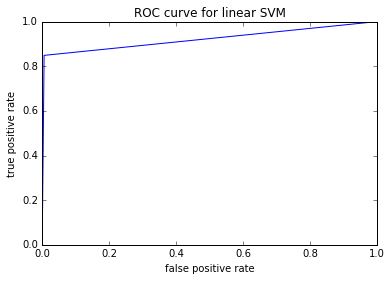
\includegraphics[width=\textwidth]{ROC_SVM.png}
	\caption{ROC curve for linear SVM}
\end{figure}

\begin{table}[h]
	\centering
	\begin{tabular}{|c|c|c|c|} \hline
		& Accuracy 		Predicted Computer Technology & Predicted Recreation Activity \\ \hline
		Actual Computer Technology & 1581 & 9 \\
		Actual Recreation Activity & 236& 1324  \\
		\hline
	\end{tabular}
	\caption{Confusion Matrix: Linear SVM}
	\label{table:ovr_res}
\end{table}

\begin{table}[h]
	\centering
	\begin{tabular}{|c|c|c|c|} \hline
		Learning Algorithm & Accuracy & Precision & Recall\\ \hline
		Linear SVM & 92.22 & 99.32 & 84.87 \\
		\hline
	\end{tabular}
	\caption{Liner SVM}
	\label{table:ovr_res}
\end{table}

\subsection{Part F: Soft Margin SVM}

\begin{figure}[h]
	
	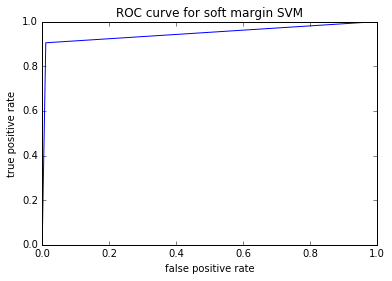
\includegraphics[width=\textwidth]{ROC_SMSVM.png}
	\caption{ROC curve for soft margin SVM}
\end{figure}

\begin{table}[h]
	\centering
	\begin{tabular}{|c|c|c|c|} \hline
		& Accuracy 		Predicted Computer Technology & Predicted Recreation Activity \\ \hline
		Actual Computer Technology & 1573 & 17 \\
		Actual Recreation Activity & 148& 1412  \\
		\hline
	\end{tabular}
	\caption{Confusion Matrix: soft margin SVM}
	\label{table:ovr_res}
\end{table}

\begin{table}[h]
	\centering
	\begin{tabular}{|c|c|c|c|} \hline
		Learning Algorithm & Accuracy & Precision & Recall\\ \hline
		Soft margin SVM & 94.76 & 98.81 & 90.51 \\
		\hline
	\end{tabular}
	\caption{soft margin SVM}
	\label{table:ovr_res}
\end{table}

\subsection{Part G Naive Bayes}

\begin{figure}[h]
	
	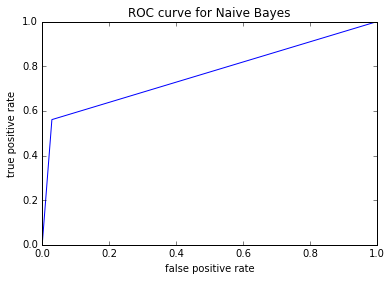
\includegraphics[width=\textwidth]{ROC_NaiveBayes.png}
	\caption{ROC curve for Naive Bayes}
\end{figure}

\begin{table}[h]
	\centering
	\begin{tabular}{|c|c|c|c|} \hline
		& Accuracy 		Predicted Computer Technology & Predicted Recreation Activity \\ \hline
		Actual Computer Technology & 1544 & 46 \\
		Actual Recreation Activity & 685& 875  \\
		\hline
	\end{tabular}
	\caption{Confusion Matrix: Naive Bayes}
	\label{table:ovr_res}
\end{table}

\begin{table}[h]
	\centering
	\begin{tabular}{|c|c|c|c|} \hline
		Learning Algorithm & Accuracy & Precision & Recall\\ \hline
		Gaussian Naive Bayes& 76.79 & 95.00 & 56.08 \\
		\hline
	\end{tabular}
	\caption{Naive Bayes}
	\label{table:ovr_res}
\end{table}

\subsection{Part G Naive Bayes}

\begin{figure}[h]
	
	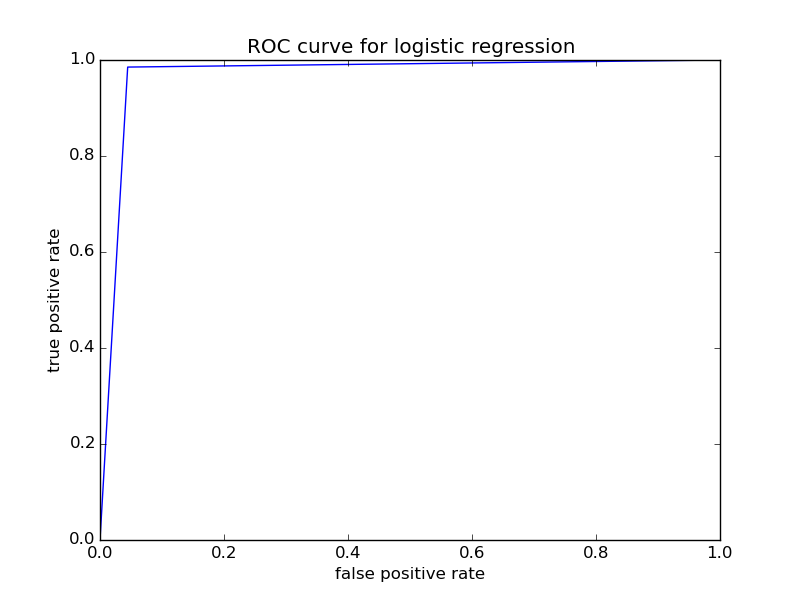
\includegraphics[width=\textwidth]{ROC_LogisticRegression.png}
	\caption{ROC curve for Logistic Regression}
\end{figure}

\begin{table}[h]
	\centering
	\begin{tabular}{|c|c|c|c|} \hline
		& Accuracy 		Predicted Computer Technology & Predicted Recreation Activity \\ \hline
		Actual Computer Technology & 1519 & 71 \\
		Actual Recreation Activity & 23& 1537  \\
		\hline
	\end{tabular}
	\caption{Confusion Matrix: Logistic Regression}
	\label{table:ovr_res}
\end{table}

\begin{table}[h]
	\centering
	\begin{tabular}{|c|c|c|c|} \hline
		Learning Algorithm & Accuracy & Precision & Recall\\ \hline
		Logistic Regression& 97.01 & 95.58 & 98.52 \\
		\hline
	\end{tabular}
	\caption{Logistic Regression}
	\label{table:ovr_res}
\end{table}




\section{Multi-class Classification}
\subsection{Part I}

The results for Multi-class classification are shown in the tables below. Table \ref{table:ovr_res} contains the results for One vs Rest method and Table \ref{table:ovo_res} contains the results for One vs One method.

\begin{table}[h]
	\centering
	\begin{tabular}{|c|c|c|c|} \hline
		Learning Algorithm & Accuracy & Precision & Recall\\ \hline
		Gaussian Naive Bayes & 63.32 & 64.50 & 63.32 \\
		Linear SVM & 81.40 & 81.50 & 81.40 \\
		\hline
		\end{tabular}
		\caption{One vs Rest}
		\label{table:ovr_res}
\end{table}

\begin{table}[h]
	\centering
	\begin{tabular}{|c|c|c|c|} \hline
		Learning Algorithm & Accuracy & Precision & Recall\\ \hline
		Gaussian Naive Bayes & 64.53 & 65.47 & 64.53 \\
		Linear SVM & 80.89 & 81.28 & 80.89 \\
		\hline
	\end{tabular}
	\caption{One vs One}
	\label{table:ovo_res}
\end{table}

\newpage
The confusion matrix for One vs One methods are shown below in figure \ref{fig:cm_ovo} and Confusion matrix for One vs Rest methods are in figure \ref{fig:cm_ovr}

\begin{figure}[h]
	
	\begin{subfigure}[b]{0.5\textwidth}
		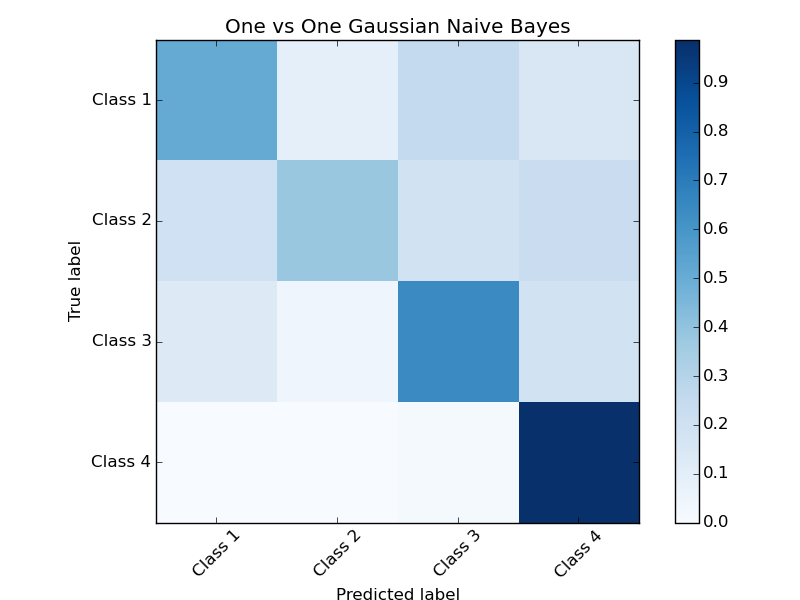
\includegraphics[width=\textwidth]{ovo_gnb.png}
		\caption{Gaussian Naive Bayes}
	\end{subfigure}
	%
	\begin{subfigure}[b]{0.5\textwidth}
		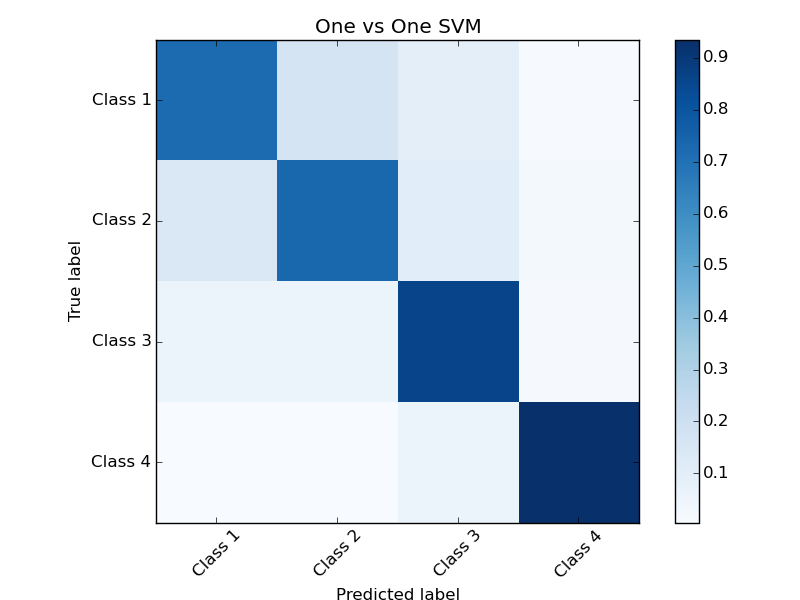
\includegraphics[width=\textwidth]{ovo_svm.png}
		\caption{Linear SVM}
	\end{subfigure}
	\caption{Confusion Matrix for One vs One Method}
	\label{fig:cm_ovo}
\end{figure}

\begin{figure}[h]
	
	\begin{subfigure}[b]{0.5\textwidth}
		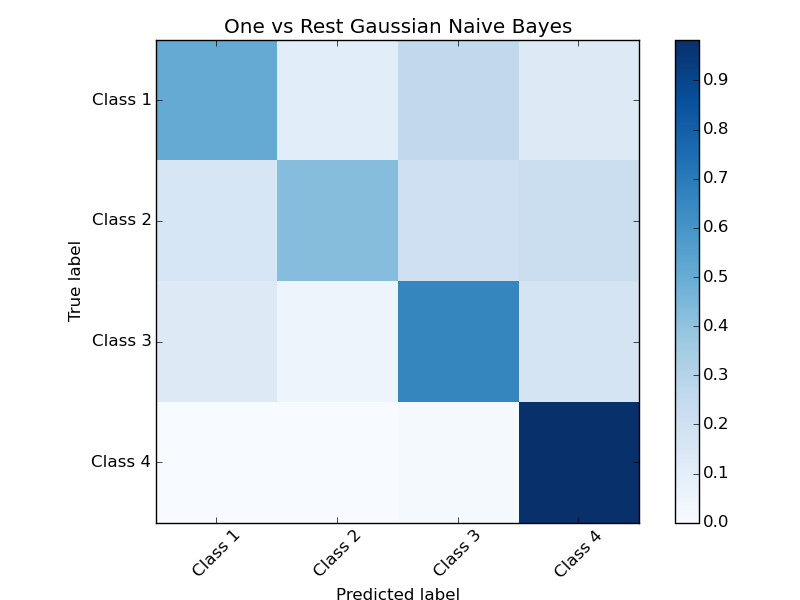
\includegraphics[width=\textwidth]{ovr_gnb.png}
		\caption{Gaussian Naive Bayes}
	\end{subfigure}
	%
	\begin{subfigure}[b]{0.5\textwidth}
		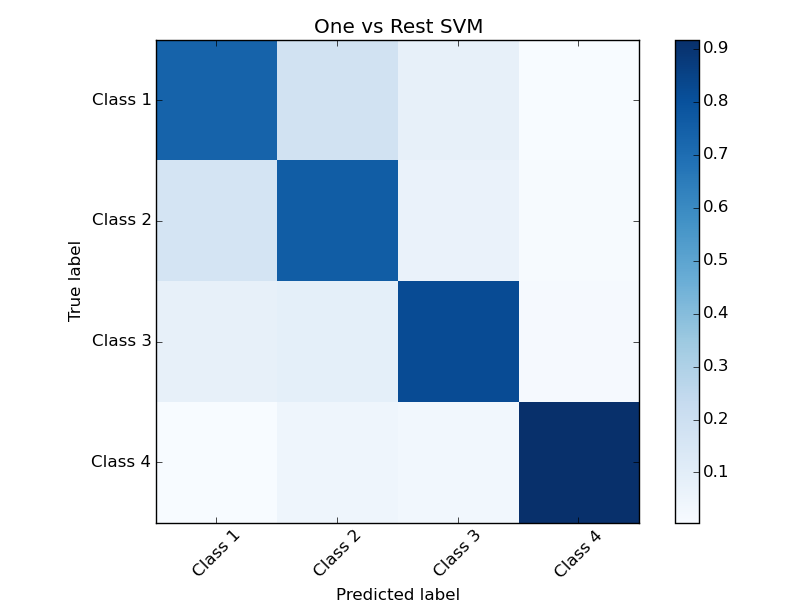
\includegraphics[width=\textwidth]{ovr_svm.png}
		\caption{Linear SVM}
	\end{subfigure}
	\caption{Confusion Matrix for One vs Rest Method}
	\label{fig:cm_ovr}
\end{figure}

\end{document}